\definecolor{lightgreen}{HTML}{E6FFFA} 
\definecolor{tablehighlight}{HTML}{D5F5E3} 
\begin{table*}[h]
    \centering
    \small
    \setlength{\tabcolsep}{3.2pt}
    \renewcommand{\arraystretch}{1.2} % Slightly increase row height for readability
    \begin{tabular}{l|ccc|cc}
    \toprule
    \multirow{2}{*}{\makecell[c]{\normalsize\textbf{Methods}}} & \multicolumn{3}{c|}{\textbf{Hallucination}} & \multicolumn{2}{c}{\textbf{Reasoning}} \\
    \cmidrule(lr){2-4} \cmidrule(lr){5-6}
    & \small\textbf{TruthfulQA} & \small\textbf{SimpleQA} & \small\textbf{ChineseSimpleQA}  & 
    \small\textbf{GPQA Diamond} & \small\textbf{AIME 2025}\\
   
    \midrule
    \multicolumn{6}{c}{\textbf{Skywork-OR1-7B-Preview}} \\
    \text{Direct Generation}     & 34.39 & 5.19 & 13.27  & 31.31 & 6.67  \\
    %\text{COT}                   & 35.01 & 5.11 & 9.50   & 39.90 & 23.33  \\
    \text{Self-Refine}           & 30.00 & 2.90 & 11.57  & 46.97 & 36.67 \\
    %\text{SC}                    & 34.64 & 6.34 & 15.77  & 41.41 & 26.67  \\
    \text{FactTune-FS}           & 34.76 & 5.33 & 12.30 & 32.83 & 6.67  \\
    \text{DPO}                   & 34.64 & 4.60 & 15.57 & 34.34 & 6.67 \\
    \text{SFT}                   & \textbf{38.43} & 4.90 & 14.87 & 32.32 & 16.67  \\
    %\midrule
    \rowcolor{tablehighlight} % Changed color here
    \text{KnowRL-Zero}           & 34.39 & \textbf{5.55} & 15.17 & 30.30 & 10.00  \\
    %\text{ColdStart}             & 35.99 & 5.14 & 14.67 & 33.84 & 20.00   \\
    %\text{ColdStart+SFT}         & 36.11 & 4.58 & 14.87 & 30.30 & 16.67 \\
    %\text{ColdStart+DPO}         & 32.68 & 4.53 & 11.77 & 36.36 & 13.33  \\
    \rowcolor{tablehighlight} % Changed color here
    \text{KnowRL}      & 37.70 & 4.58 & \textbf{16.23} & 34.34$\uparrow$ & 10.00$\uparrow$ \\
       
    \midrule
        \multicolumn{6}{c}{\textbf{DeepSeek-R1-Distill-Qwen-7B}} \\
    \text{Direct Generation}     & 33.05 & 1.92 & 11.17  & 34.34 & 16.67  \\
    %\text{COT}                   & 32.80 & 2.55 & 11.53  & 41.41 & 30.00  \\
    \text{Self-Refine}           & 33.90 & 2.60 & 9.97   & 45.45 & 33.33  \\
    %\text{SC}                    & 34.88 & 3.04 & 11.47  & 42.42 &  23.33 \\
    \text{FactTune-FS}           & 35.50 & 2.46 & 10.27 & 36.87 & 26.67  \\
    \text{DPO}                   & 36.96 & 3.21 & 12.33 & 37.37 & 13.33  \\
    \text{SFT}                   & 37.09 & 4.12 & 12.70 & 30.30 & 16.67    \\
    %\midrule
    \rowcolor{tablehighlight} % Changed color here
    \text{KnowRL-Zero}            & 33.54 & 1.34 & 11.00 & 34.34 & 6.67  \\
    %\text{ColdStart}             & 35.86 & 3.75 & 12.70 & 39.39 & 20.00   \\
    %\text{ColdStart+SFT}         & 37.21 & 3.59 & 13.47 & 31.31 & 16.67 \\
    %\text{ColdStart+DPO}         & 33.41 & 3.34 & 10.63 & 33.84 & 6.67  \\
    \rowcolor{tablehighlight} % Changed color here
    \text{KnowRL}      & \textbf{38.19} & \textbf{4.56} & \textbf{13.90} & 37.37$\uparrow$ &  13.33$\downarrow$ \\
    
    
    \bottomrule
    \end{tabular}
    \vspace{-1ex}
    \caption{\textbf{Main Experiment.} KnowRL-Zero is a method of RL training without cold-start training. KnowRL represents RL training on a cold-start trained model. The best results are marked in \textbf{bold}.}
    \vspace{-3ex}
    \label{main-exp}
\end{table*}

\begin{figure*}[!htbp]
    \centering
    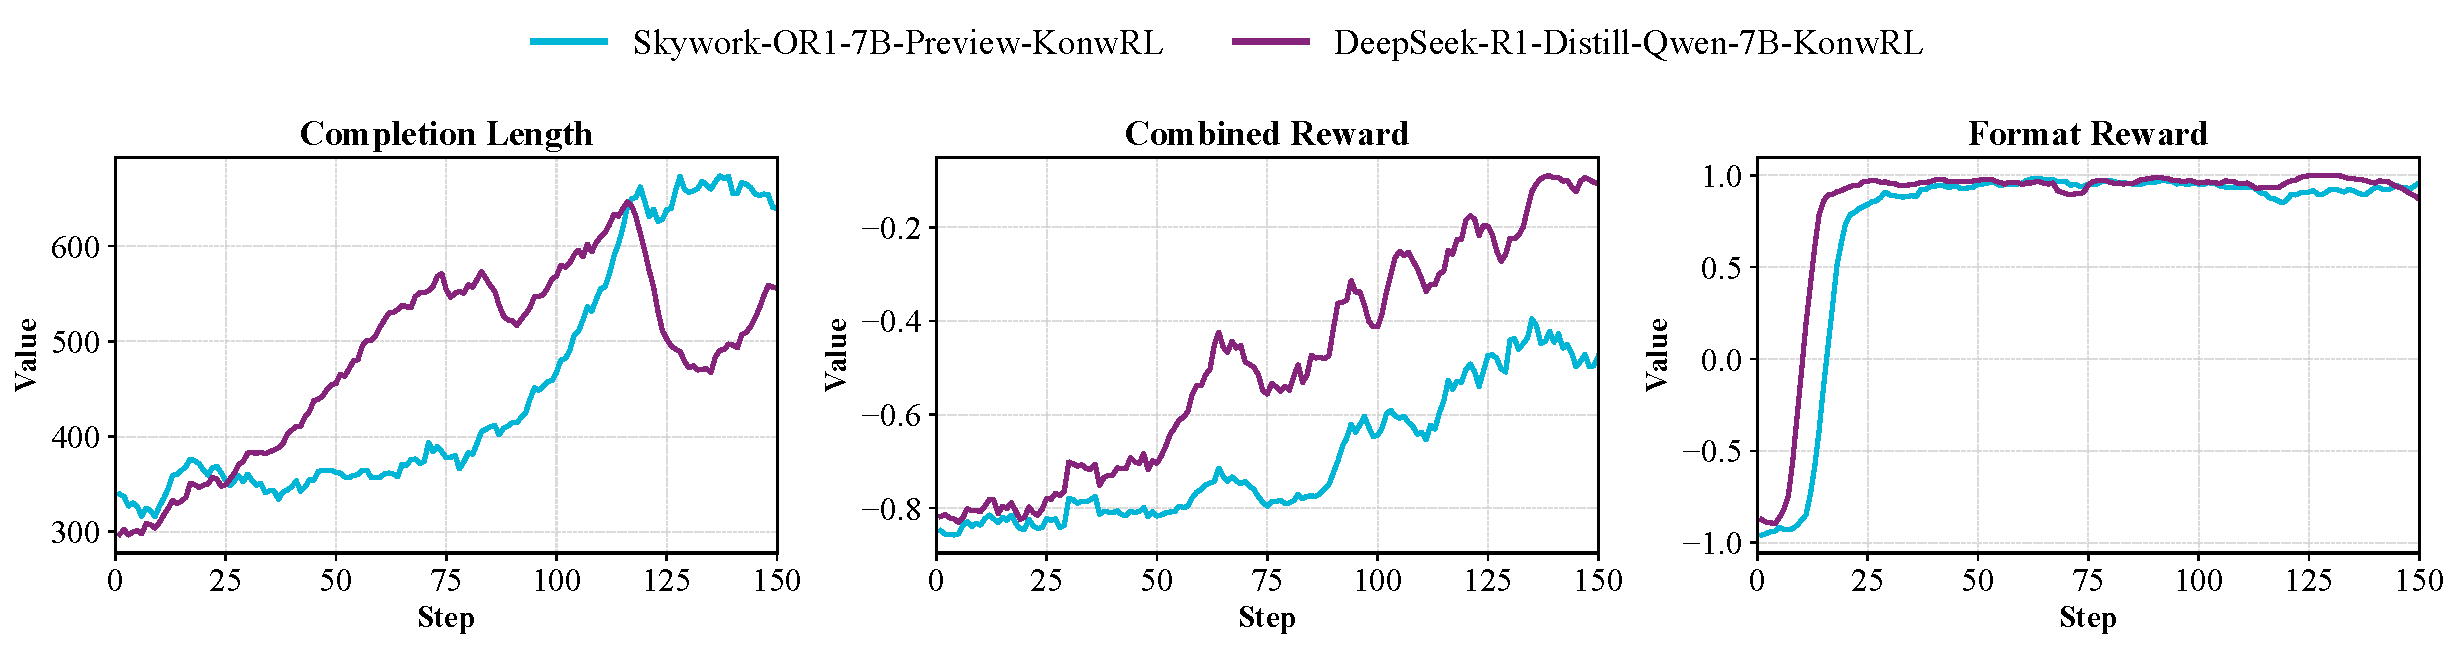
\includegraphics[width=1\linewidth]{images/rl_training_curves_comparison.pdf}
    % \vspace{-2ex}
    \caption{\textbf{KnowRL Training Curve.} The Combined Reward is $R_{combined}$.}
    \vspace{-3ex}
    \label{knowrl-exp}
\end{figure*}



\begin{table*}[t]
    \centering
    \small
    \setlength{\tabcolsep}{3.2pt}
    \renewcommand{\arraystretch}{1.2}
    % Define table structure: 3 cols for rewards, 3 for Hallucination, 2 for Reasoning
    \begin{tabular}{ccc|ccc|cc}
    \toprule
    % Main header row
    \multicolumn{3}{c|}{\textbf{Reward}} & \multicolumn{3}{c|}{\textbf{Hallucination}} & \multicolumn{2}{c}{\textbf{Reasoning}} \\
    \cmidrule(lr){4-6} \cmidrule(lr){7-8}
    % Sub-header row
    \textbf{$R_{format}$} & \textbf{$R_{fact}$} & \textbf{$R_{correct}$} & \small\textbf{TruthfulQA} & \small\textbf{SimpleQA} & \small\textbf{ChineseSimpleQA} &
    \small\textbf{GPQA Diamond} & \small\textbf{AIME 2025}\\

    \midrule
    \multicolumn{8}{c}{\textbf{DeepSeek-R1-Distill-Qwen-7B}} \\
   
    \checkmark & \ding{55} & \ding{55} & 33.41 & \textbf{2.36} & 10.47  & 35.86 & 10.00  \\
    \checkmark & \checkmark & \ding{55} & 34.03 & 1.55 & 9.70  & 31.31 & 16.67  \\
    \checkmark & \ding{55} & \checkmark & \textbf{34.76}  & 1.74 & 10.97 & \textbf{37.88} & \textbf{20.00}  \\
    \rowcolor{tablehighlight}
    \checkmark & \checkmark & \checkmark & 33.54 & 1.34 & \textbf{11.00} & 34.34 & 6.67  \\
        
    \midrule
    \multicolumn{8}{c}{\textbf{DeepSeek-R1-Distill-Qwen-7B-ColdStart}} \\
  
    \checkmark & \ding{55} & \ding{55} & 36.84 & 3.73 & 14.37 & 35.86 & \textbf{16.67}  \\
    \checkmark & \checkmark & \ding{55} & 37.82 & \textbf{6.16} & \textbf{14.60} & 35.86 & 13.33 \\
    \checkmark & \ding{55} & \checkmark & 37.82 & 4.04 & 13.80 & 33.33 & \textbf{16.67} \\
    \rowcolor{tablehighlight}
    \checkmark & \checkmark & \checkmark & \textbf{38.19} & 4.56 & 13.90 & \textbf{37.37} & 13.33 \\
    
    \bottomrule
    \end{tabular}
    \vspace{-1ex}
    \caption{\textbf{Reward Ablation Experiment.} DeepSeek-R1-Distill-Qwen-7B is trained with cold start to obtain DeepSeek-R1-Distill-Qwen-7B-ColdStart. The best results are marked in \textbf{bold}.
     For the reward components, \checkmark indicates inclusion and \ding{55} indicates exclusion.
    }
    \vspace{-3ex}
    \label{ablation}
\end{table*}


\begin{figure*}[t]
    \centering
     \vspace{2ex}
    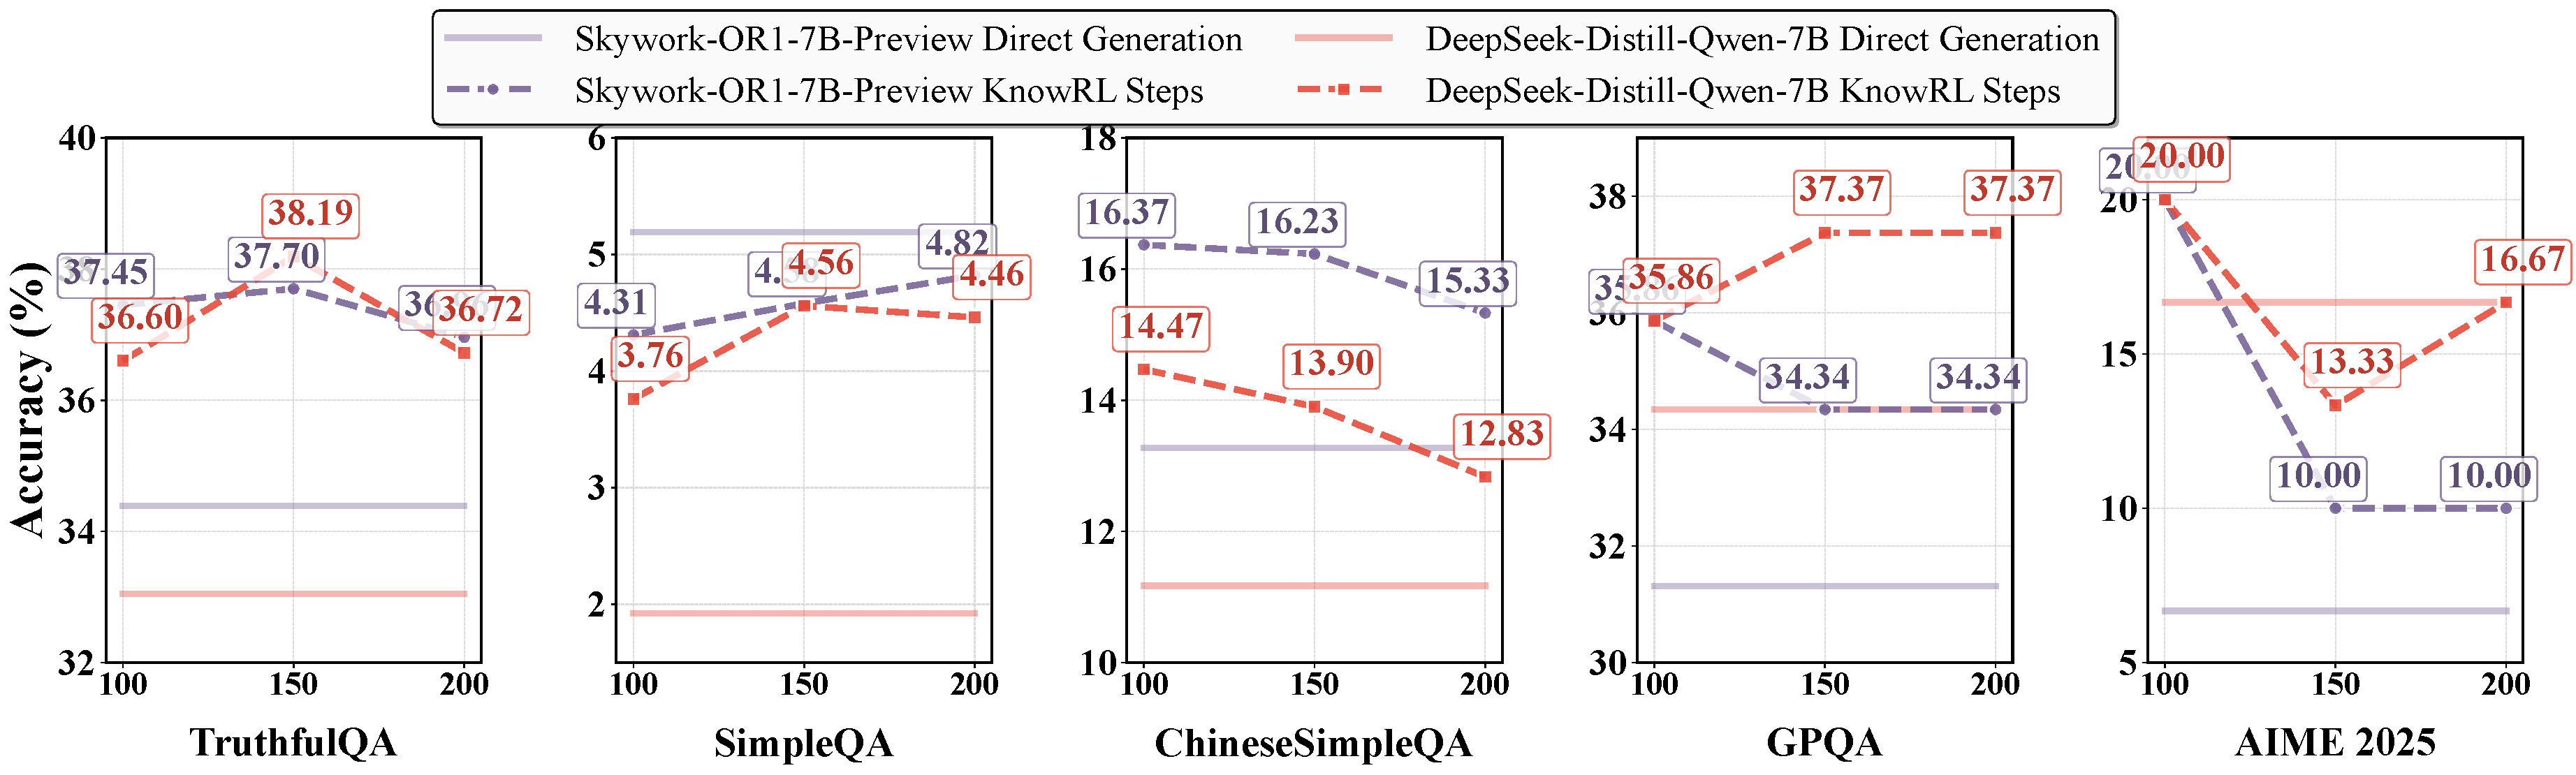
\includegraphics[width=0.95\linewidth]{images/trainstep_two_models.pdf}
    \caption{Performance of the Skywork-OR1-7B-Preview and DeepSeek-R1-Distill-Qwen-7B on 5 datasets with different number of training steps.}
    \vspace{-4ex}
    \label{train-step1}
\end{figure*}


